% Options for packages loaded elsewhere
% Options for packages loaded elsewhere
\PassOptionsToPackage{unicode}{hyperref}
\PassOptionsToPackage{hyphens}{url}
\PassOptionsToPackage{dvipsnames,svgnames,x11names}{xcolor}
%
\documentclass[
  letterpaper,
  DIV=11,
  numbers=noendperiod]{scrartcl}
\usepackage{xcolor}
\usepackage{amsmath,amssymb}
\setcounter{secnumdepth}{5}
\usepackage{iftex}
\ifPDFTeX
  \usepackage[T1]{fontenc}
  \usepackage[utf8]{inputenc}
  \usepackage{textcomp} % provide euro and other symbols
\else % if luatex or xetex
  \usepackage{unicode-math} % this also loads fontspec
  \defaultfontfeatures{Scale=MatchLowercase}
  \defaultfontfeatures[\rmfamily]{Ligatures=TeX,Scale=1}
\fi
\usepackage{lmodern}
\ifPDFTeX\else
  % xetex/luatex font selection
\fi
% Use upquote if available, for straight quotes in verbatim environments
\IfFileExists{upquote.sty}{\usepackage{upquote}}{}
\IfFileExists{microtype.sty}{% use microtype if available
  \usepackage[]{microtype}
  \UseMicrotypeSet[protrusion]{basicmath} % disable protrusion for tt fonts
}{}
\makeatletter
\@ifundefined{KOMAClassName}{% if non-KOMA class
  \IfFileExists{parskip.sty}{%
    \usepackage{parskip}
  }{% else
    \setlength{\parindent}{0pt}
    \setlength{\parskip}{6pt plus 2pt minus 1pt}}
}{% if KOMA class
  \KOMAoptions{parskip=half}}
\makeatother
% Make \paragraph and \subparagraph free-standing
\makeatletter
\ifx\paragraph\undefined\else
  \let\oldparagraph\paragraph
  \renewcommand{\paragraph}{
    \@ifstar
      \xxxParagraphStar
      \xxxParagraphNoStar
  }
  \newcommand{\xxxParagraphStar}[1]{\oldparagraph*{#1}\mbox{}}
  \newcommand{\xxxParagraphNoStar}[1]{\oldparagraph{#1}\mbox{}}
\fi
\ifx\subparagraph\undefined\else
  \let\oldsubparagraph\subparagraph
  \renewcommand{\subparagraph}{
    \@ifstar
      \xxxSubParagraphStar
      \xxxSubParagraphNoStar
  }
  \newcommand{\xxxSubParagraphStar}[1]{\oldsubparagraph*{#1}\mbox{}}
  \newcommand{\xxxSubParagraphNoStar}[1]{\oldsubparagraph{#1}\mbox{}}
\fi
\makeatother

\usepackage{color}
\usepackage{fancyvrb}
\newcommand{\VerbBar}{|}
\newcommand{\VERB}{\Verb[commandchars=\\\{\}]}
\DefineVerbatimEnvironment{Highlighting}{Verbatim}{commandchars=\\\{\}}
% Add ',fontsize=\small' for more characters per line
\usepackage{framed}
\definecolor{shadecolor}{RGB}{241,243,245}
\newenvironment{Shaded}{\begin{snugshade}}{\end{snugshade}}
\newcommand{\AlertTok}[1]{\textcolor[rgb]{0.68,0.00,0.00}{#1}}
\newcommand{\AnnotationTok}[1]{\textcolor[rgb]{0.37,0.37,0.37}{#1}}
\newcommand{\AttributeTok}[1]{\textcolor[rgb]{0.40,0.45,0.13}{#1}}
\newcommand{\BaseNTok}[1]{\textcolor[rgb]{0.68,0.00,0.00}{#1}}
\newcommand{\BuiltInTok}[1]{\textcolor[rgb]{0.00,0.23,0.31}{#1}}
\newcommand{\CharTok}[1]{\textcolor[rgb]{0.13,0.47,0.30}{#1}}
\newcommand{\CommentTok}[1]{\textcolor[rgb]{0.37,0.37,0.37}{#1}}
\newcommand{\CommentVarTok}[1]{\textcolor[rgb]{0.37,0.37,0.37}{\textit{#1}}}
\newcommand{\ConstantTok}[1]{\textcolor[rgb]{0.56,0.35,0.01}{#1}}
\newcommand{\ControlFlowTok}[1]{\textcolor[rgb]{0.00,0.23,0.31}{\textbf{#1}}}
\newcommand{\DataTypeTok}[1]{\textcolor[rgb]{0.68,0.00,0.00}{#1}}
\newcommand{\DecValTok}[1]{\textcolor[rgb]{0.68,0.00,0.00}{#1}}
\newcommand{\DocumentationTok}[1]{\textcolor[rgb]{0.37,0.37,0.37}{\textit{#1}}}
\newcommand{\ErrorTok}[1]{\textcolor[rgb]{0.68,0.00,0.00}{#1}}
\newcommand{\ExtensionTok}[1]{\textcolor[rgb]{0.00,0.23,0.31}{#1}}
\newcommand{\FloatTok}[1]{\textcolor[rgb]{0.68,0.00,0.00}{#1}}
\newcommand{\FunctionTok}[1]{\textcolor[rgb]{0.28,0.35,0.67}{#1}}
\newcommand{\ImportTok}[1]{\textcolor[rgb]{0.00,0.46,0.62}{#1}}
\newcommand{\InformationTok}[1]{\textcolor[rgb]{0.37,0.37,0.37}{#1}}
\newcommand{\KeywordTok}[1]{\textcolor[rgb]{0.00,0.23,0.31}{\textbf{#1}}}
\newcommand{\NormalTok}[1]{\textcolor[rgb]{0.00,0.23,0.31}{#1}}
\newcommand{\OperatorTok}[1]{\textcolor[rgb]{0.37,0.37,0.37}{#1}}
\newcommand{\OtherTok}[1]{\textcolor[rgb]{0.00,0.23,0.31}{#1}}
\newcommand{\PreprocessorTok}[1]{\textcolor[rgb]{0.68,0.00,0.00}{#1}}
\newcommand{\RegionMarkerTok}[1]{\textcolor[rgb]{0.00,0.23,0.31}{#1}}
\newcommand{\SpecialCharTok}[1]{\textcolor[rgb]{0.37,0.37,0.37}{#1}}
\newcommand{\SpecialStringTok}[1]{\textcolor[rgb]{0.13,0.47,0.30}{#1}}
\newcommand{\StringTok}[1]{\textcolor[rgb]{0.13,0.47,0.30}{#1}}
\newcommand{\VariableTok}[1]{\textcolor[rgb]{0.07,0.07,0.07}{#1}}
\newcommand{\VerbatimStringTok}[1]{\textcolor[rgb]{0.13,0.47,0.30}{#1}}
\newcommand{\WarningTok}[1]{\textcolor[rgb]{0.37,0.37,0.37}{\textit{#1}}}

\usepackage{longtable,booktabs,array}
\usepackage{calc} % for calculating minipage widths
% Correct order of tables after \paragraph or \subparagraph
\usepackage{etoolbox}
\makeatletter
\patchcmd\longtable{\par}{\if@noskipsec\mbox{}\fi\par}{}{}
\makeatother
% Allow footnotes in longtable head/foot
\IfFileExists{footnotehyper.sty}{\usepackage{footnotehyper}}{\usepackage{footnote}}
\makesavenoteenv{longtable}
\usepackage{graphicx}
\makeatletter
\newsavebox\pandoc@box
\newcommand*\pandocbounded[1]{% scales image to fit in text height/width
  \sbox\pandoc@box{#1}%
  \Gscale@div\@tempa{\textheight}{\dimexpr\ht\pandoc@box+\dp\pandoc@box\relax}%
  \Gscale@div\@tempb{\linewidth}{\wd\pandoc@box}%
  \ifdim\@tempb\p@<\@tempa\p@\let\@tempa\@tempb\fi% select the smaller of both
  \ifdim\@tempa\p@<\p@\scalebox{\@tempa}{\usebox\pandoc@box}%
  \else\usebox{\pandoc@box}%
  \fi%
}
% Set default figure placement to htbp
\def\fps@figure{htbp}
\makeatother





\setlength{\emergencystretch}{3em} % prevent overfull lines

\providecommand{\tightlist}{%
  \setlength{\itemsep}{0pt}\setlength{\parskip}{0pt}}



 


\KOMAoption{captions}{tableheading}
\makeatletter
\@ifpackageloaded{caption}{}{\usepackage{caption}}
\AtBeginDocument{%
\ifdefined\contentsname
  \renewcommand*\contentsname{Table of contents}
\else
  \newcommand\contentsname{Table of contents}
\fi
\ifdefined\listfigurename
  \renewcommand*\listfigurename{List of Figures}
\else
  \newcommand\listfigurename{List of Figures}
\fi
\ifdefined\listtablename
  \renewcommand*\listtablename{List of Tables}
\else
  \newcommand\listtablename{List of Tables}
\fi
\ifdefined\figurename
  \renewcommand*\figurename{Figure}
\else
  \newcommand\figurename{Figure}
\fi
\ifdefined\tablename
  \renewcommand*\tablename{Table}
\else
  \newcommand\tablename{Table}
\fi
}
\@ifpackageloaded{float}{}{\usepackage{float}}
\floatstyle{ruled}
\@ifundefined{c@chapter}{\newfloat{codelisting}{h}{lop}}{\newfloat{codelisting}{h}{lop}[chapter]}
\floatname{codelisting}{Listing}
\newcommand*\listoflistings{\listof{codelisting}{List of Listings}}
\makeatother
\makeatletter
\makeatother
\makeatletter
\@ifpackageloaded{caption}{}{\usepackage{caption}}
\@ifpackageloaded{subcaption}{}{\usepackage{subcaption}}
\makeatother
\usepackage{bookmark}
\IfFileExists{xurl.sty}{\usepackage{xurl}}{} % add URL line breaks if available
\urlstyle{same}
\hypersetup{
  pdftitle={Data Science Replication Study},
  pdfauthor={Team A},
  colorlinks=true,
  linkcolor={blue},
  filecolor={Maroon},
  citecolor={Blue},
  urlcolor={Blue},
  pdfcreator={LaTeX via pandoc}}


\title{Data Science Replication Study}
\author{Team A}
\date{}
\begin{document}
\maketitle

\renewcommand*\contentsname{Table of contents}
{
\hypersetup{linkcolor=}
\setcounter{tocdepth}{3}
\tableofcontents
}

\section{Data Science for Business}\label{data-science-for-business}

\subsection{Team A:}\label{team-a}

\subsubsection{Mohamad Abdulla}\label{mohamad-abdulla}

\subsubsection{Anvith Amin}\label{anvith-amin}

\subsubsection{Manjunath Mallikarjun
Kendhuli}\label{manjunath-mallikarjun-kendhuli}

\begin{center}\rule{0.5\linewidth}{0.5pt}\end{center}

\section{Papers Reviewed}\label{papers-reviewed}

\begin{itemize}
\tightlist
\item
  Paper 1: Predicting Employee Attrition (IBM)
\item
  Paper 2: Data Analytics for Optimizing and Predicting Employee
  Performance
\item
  Paper 3: Migration and Innovation: Learning from Patent and Inventor
  Data
\item
  Challenges faced during the project
\end{itemize}

\begin{center}\rule{0.5\linewidth}{0.5pt}\end{center}

\section{Selected Paper}\label{selected-paper}

\subsection{``The Political Economy of Green Industrial
Policy''}\label{the-political-economy-of-green-industrial-policy}

\emph{Juhász et al., 2022}

\begin{itemize}
\tightlist
\item
  Used Global Trade Alert (GTA) database
\item
  Three key figures showing green policy trends in G20 countries
\end{itemize}

\begin{center}\rule{0.5\linewidth}{0.5pt}\end{center}

\section{Problems Faced}\label{problems-faced}

\begin{itemize}
\tightlist
\item
  Unclear objectives at the beginning
\item
  Extremely large and complex datasets
\item
  GitHub deployment issues
\end{itemize}

\begin{center}\rule{0.5\linewidth}{0.5pt}\end{center}

\section{Replication of Figure 1}\label{replication-of-figure-1}

\begin{itemize}
\tightlist
\item
  \textbf{Title:} Green Industrial Policy Activity in G20 Countries
  (2010--2022)
\item
  \textbf{What it shows:}

  \begin{itemize}
  \tightlist
  \item
    Annual green policy activity for Middle-income vs.~High-income
    countries
  \item
    Indexed to 2010--2012 average = 100
  \item
    High-income line is scaled (divided by 5) for visual comparison
  \end{itemize}
\item
  \textbf{Axes:}

  \begin{itemize}
  \tightlist
  \item
    Left Y-axis: Middle-income index\\
  \item
    Right Y-axis: High-income index (scaled)
  \end{itemize}
\end{itemize}

\begin{center}\rule{0.5\linewidth}{0.5pt}\end{center}

\section{Replication Figure}\label{replication-figure}

\begin{figure}[H]

{\centering 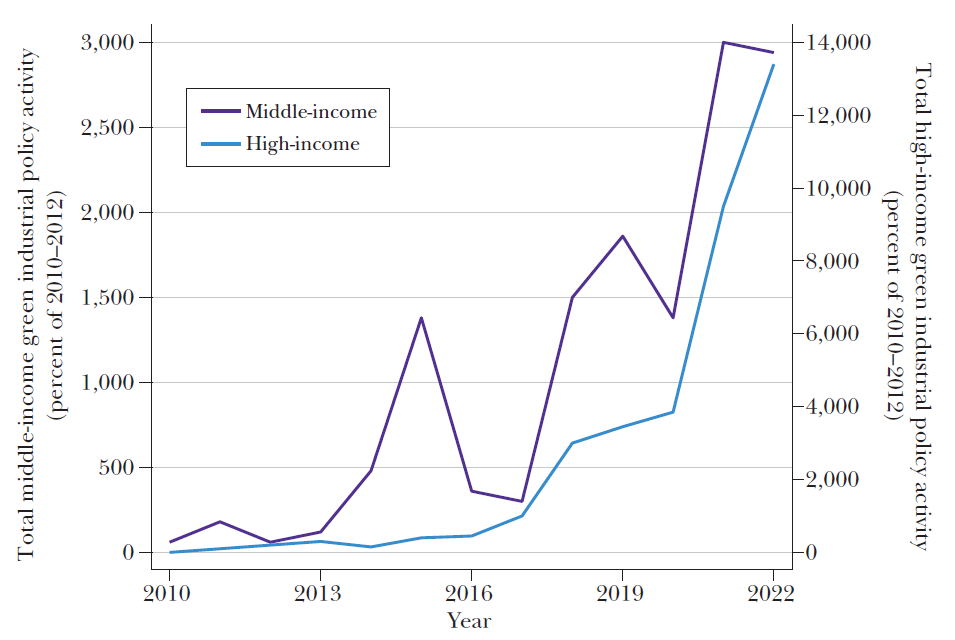
\includegraphics[width=1\linewidth,height=\textheight,keepaspectratio]{index_files/mediabag/figure_1.png}

}

\caption{Fig 1: Green Industrial Policy Activity in G20 Countries,
2010--2022}

\end{figure}%

\begin{center}\rule{0.5\linewidth}{0.5pt}\end{center}

\section{Code Logic Summary}\label{code-logic-summary}

\begin{itemize}
\tightlist
\item
  \textbf{Step 1: Load and clean raw data}

  \begin{itemize}
  \tightlist
  \item
    Import original \texttt{IP\_G20.dta} file\\
  \item
    Filter valid rows and deduplicate by MeasureID--Year--Country
  \end{itemize}
\item
  \textbf{Step 2: Identify green policies}

  \begin{itemize}
  \tightlist
  \item
    Use keywords like \emph{climate, emission, renewable} to flag green
    measures
  \end{itemize}
\item
  \textbf{Step 3: Add income group classification}

  \begin{itemize}
  \tightlist
  \item
    Load World Bank Excel data\\
  \item
    Reshape to long format and convert fiscal to calendar years\\
  \item
    Merge with green policy data by country and year
  \end{itemize}
\end{itemize}

\begin{center}\rule{0.5\linewidth}{0.5pt}\end{center}

\begin{itemize}
\tightlist
\item
  \textbf{Step 4: Standardize income group labels}

  \begin{itemize}
  \tightlist
  \item
    Map \texttt{H} to ``High-income'', \texttt{LM/UM} to
    ``Middle-income''\\
  \item
    Remove unmatched or missing classifications
  \end{itemize}
\item
  \textbf{Step 5: Count policies per year}

  \begin{itemize}
  \tightlist
  \item
    Group by year and income group\\
  \item
    Count number of green policies announced
  \end{itemize}
\item
  \textbf{Step 6: Compute 2010--2012 baseline}

  \begin{itemize}
  \tightlist
  \item
    Calculate average policy count in 2010--2012 for each group
  \end{itemize}
\item
  \textbf{Step 7: Index calculation}

  \begin{itemize}
  \tightlist
  \item
    Create index: \texttt{(policy\_count\ /\ baseline\_avg)\ *\ 100}\\
  \item
    Expresses annual activity relative to baseline (baseline = 100)
  \end{itemize}
\end{itemize}

\begin{center}\rule{0.5\linewidth}{0.5pt}\end{center}

\begin{itemize}
\tightlist
\item
  \textbf{Step 8: Visualization}

  \begin{itemize}
  \tightlist
  \item
    Plot both income groups on one chart\\
  \item
    Scale high-income index by \texttt{/5} on secondary Y-axis for
    comparison
  \end{itemize}
\end{itemize}

\begin{center}\rule{0.5\linewidth}{0.5pt}\end{center}

\section{R Code for Replication}\label{r-code-for-replication}

\begin{Shaded}
\begin{Highlighting}[]
\CommentTok{\# {-}{-}{-}{-}{-}{-}{-}{-}{-}{-}{-}{-}{-}{-}{-}{-}{-}{-}{-}{-}{-}{-}{-}{-}{-}{-}{-}{-}{-}{-}{-}}
\CommentTok{\# STEP 1: Load Required Libraries}
\CommentTok{\# {-}{-}{-}{-}{-}{-}{-}{-}{-}{-}{-}{-}{-}{-}{-}{-}{-}{-}{-}{-}{-}{-}{-}{-}{-}{-}{-}{-}{-}{-}{-}}
\ControlFlowTok{if}\NormalTok{ (}\SpecialCharTok{!}\FunctionTok{require}\NormalTok{(pacman)) }\FunctionTok{install.packages}\NormalTok{(}\StringTok{"pacman"}\NormalTok{)}
\end{Highlighting}
\end{Shaded}

\begin{verbatim}
Loading required package: pacman
\end{verbatim}

\begin{Shaded}
\begin{Highlighting}[]
\NormalTok{pacman}\SpecialCharTok{::}\FunctionTok{p\_unload}\NormalTok{(all)}
\end{Highlighting}
\end{Shaded}

\begin{verbatim}
The following packages have been unloaded:
pacman
\end{verbatim}

\begin{Shaded}
\begin{Highlighting}[]
\NormalTok{pacman}\SpecialCharTok{::}\FunctionTok{p\_load}\NormalTok{(tidyverse, haven, janitor)}

\CommentTok{\# {-}{-}{-}{-}{-}{-}{-}{-}{-}{-}{-}{-}{-}{-}{-}{-}{-}{-}{-}{-}{-}{-}{-}{-}{-}{-}{-}{-}{-}{-}{-}}
\CommentTok{\# STEP 2: Load the Raw Dataset}
\CommentTok{\# {-}{-}{-}{-}{-}{-}{-}{-}{-}{-}{-}{-}{-}{-}{-}{-}{-}{-}{-}{-}{-}{-}{-}{-}{-}{-}{-}{-}{-}{-}{-}}

\CommentTok{\# Define the correct raw URL of the .dta file}
\NormalTok{url }\OtherTok{\textless{}{-}} \StringTok{"https://raw.githubusercontent.com/anvitho07/Data{-}science{-}presentation{-}final/main/IP\_G20.dta"}

\CommentTok{\# Create a temporary local file to download the dataset}
\NormalTok{temp\_file }\OtherTok{\textless{}{-}} \FunctionTok{tempfile}\NormalTok{(}\AttributeTok{fileext =} \StringTok{".dta"}\NormalTok{)}

\CommentTok{\# Download the dataset from GitHub}
\FunctionTok{download.file}\NormalTok{(url, temp\_file, }\AttributeTok{mode =} \StringTok{"wb"}\NormalTok{)  }\CommentTok{\# use "wb" for binary files}

\CommentTok{\# Read the dataset}
\NormalTok{raw\_data }\OtherTok{\textless{}{-}} \FunctionTok{read\_dta}\NormalTok{(temp\_file)}

\CommentTok{\# {-}{-}{-}{-}{-}{-}{-}{-}{-}{-}{-}{-}{-}{-}{-}{-}{-}{-}{-}{-}{-}{-}{-}{-}{-}{-}{-}{-}{-}{-}{-}}
\CommentTok{\# STEP 3: Filter Valid Policies and Deduplicate}
\CommentTok{\#         (one row per policy{-}year{-}country combination)}
\CommentTok{\# {-}{-}{-}{-}{-}{-}{-}{-}{-}{-}{-}{-}{-}{-}{-}{-}{-}{-}{-}{-}{-}{-}{-}{-}{-}{-}{-}{-}{-}{-}{-}}
\NormalTok{green\_data }\OtherTok{\textless{}{-}}\NormalTok{ raw\_data }\SpecialCharTok{\%\textgreater{}\%}
  \FunctionTok{filter}\NormalTok{(}\SpecialCharTok{!}\FunctionTok{is.na}\NormalTok{(MeasureDescriptionTokens)) }\SpecialCharTok{\%\textgreater{}\%}
  \FunctionTok{filter}\NormalTok{(}\SpecialCharTok{!}\FunctionTok{is.na}\NormalTok{(AnnouncedYear)) }\SpecialCharTok{\%\textgreater{}\%}
  \FunctionTok{distinct}\NormalTok{(MeasureID, AnnouncedYear, CountryStd, }\AttributeTok{.keep\_all =} \ConstantTok{TRUE}\NormalTok{)}

\CommentTok{\# {-}{-}{-}{-}{-}{-}{-}{-}{-}{-}{-}{-}{-}{-}{-}{-}{-}{-}{-}{-}{-}{-}{-}{-}{-}{-}{-}{-}{-}{-}{-}}
\CommentTok{\# STEP 4: Classify Countries as High{-}income vs Middle{-}income}
\CommentTok{\#         (same static grouping as in Stata script)}
\CommentTok{\# {-}{-}{-}{-}{-}{-}{-}{-}{-}{-}{-}{-}{-}{-}{-}{-}{-}{-}{-}{-}{-}{-}{-}{-}{-}{-}{-}{-}{-}{-}{-}}
\NormalTok{high\_income }\OtherTok{\textless{}{-}} \FunctionTok{c}\NormalTok{(}\StringTok{"Australia"}\NormalTok{, }\StringTok{"Canada"}\NormalTok{, }\StringTok{"France"}\NormalTok{, }\StringTok{"Germany"}\NormalTok{, }\StringTok{"Italy"}\NormalTok{, }\StringTok{"Japan"}\NormalTok{,}
                 \StringTok{"Republic of Korea"}\NormalTok{, }\StringTok{"United Kingdom"}\NormalTok{, }\StringTok{"United States"}\NormalTok{, }\StringTok{"European Union"}\NormalTok{)}

\NormalTok{green\_data }\OtherTok{\textless{}{-}}\NormalTok{ green\_data }\SpecialCharTok{\%\textgreater{}\%}
  \FunctionTok{mutate}\NormalTok{(}\AttributeTok{IncomeGroup =} \FunctionTok{ifelse}\NormalTok{(CountryStd }\SpecialCharTok{\%in\%}\NormalTok{ high\_income, }\StringTok{"High{-}income"}\NormalTok{, }\StringTok{"Middle{-}income"}\NormalTok{))}

\CommentTok{\# {-}{-}{-}{-}{-}{-}{-}{-}{-}{-}{-}{-}{-}{-}{-}{-}{-}{-}{-}{-}{-}{-}{-}{-}{-}{-}{-}{-}{-}{-}{-}}
\CommentTok{\# STEP 5: Count Green Policies Per Year \& Group}
\CommentTok{\# {-}{-}{-}{-}{-}{-}{-}{-}{-}{-}{-}{-}{-}{-}{-}{-}{-}{-}{-}{-}{-}{-}{-}{-}{-}{-}{-}{-}{-}{-}{-}}
\NormalTok{counts }\OtherTok{\textless{}{-}}\NormalTok{ green\_data }\SpecialCharTok{\%\textgreater{}\%}
  \FunctionTok{group\_by}\NormalTok{(AnnouncedYear, IncomeGroup) }\SpecialCharTok{\%\textgreater{}\%}
  \FunctionTok{summarise}\NormalTok{(}\AttributeTok{policy\_count =} \FunctionTok{n}\NormalTok{(), }\AttributeTok{.groups =} \StringTok{"drop"}\NormalTok{)}

\CommentTok{\# {-}{-}{-}{-}{-}{-}{-}{-}{-}{-}{-}{-}{-}{-}{-}{-}{-}{-}{-}{-}{-}{-}{-}{-}{-}{-}{-}{-}{-}{-}{-}}
\CommentTok{\# STEP 6: Compute the 2010–2012 Average (Baseline Index)}
\CommentTok{\# {-}{-}{-}{-}{-}{-}{-}{-}{-}{-}{-}{-}{-}{-}{-}{-}{-}{-}{-}{-}{-}{-}{-}{-}{-}{-}{-}{-}{-}{-}{-}}
\NormalTok{baseline }\OtherTok{\textless{}{-}}\NormalTok{ counts }\SpecialCharTok{\%\textgreater{}\%}
  \FunctionTok{filter}\NormalTok{(AnnouncedYear }\SpecialCharTok{\%in\%} \DecValTok{2010}\SpecialCharTok{:}\DecValTok{2012}\NormalTok{) }\SpecialCharTok{\%\textgreater{}\%}
  \FunctionTok{group\_by}\NormalTok{(IncomeGroup) }\SpecialCharTok{\%\textgreater{}\%}
  \FunctionTok{summarise}\NormalTok{(}\AttributeTok{baseline\_avg =} \FunctionTok{mean}\NormalTok{(policy\_count), }\AttributeTok{.groups =} \StringTok{"drop"}\NormalTok{)}

\CommentTok{\# {-}{-}{-}{-}{-}{-}{-}{-}{-}{-}{-}{-}{-}{-}{-}{-}{-}{-}{-}{-}{-}{-}{-}{-}{-}{-}{-}{-}{-}{-}{-}}
\CommentTok{\# STEP 7: Calculate Index as Percent of 2010–2012 Baseline}
\CommentTok{\#         (Multiplied by 1000 to match paper\textquotesingle{}s visual scaling)}
\CommentTok{\# {-}{-}{-}{-}{-}{-}{-}{-}{-}{-}{-}{-}{-}{-}{-}{-}{-}{-}{-}{-}{-}{-}{-}{-}{-}{-}{-}{-}{-}{-}{-}}
\NormalTok{final }\OtherTok{\textless{}{-}}\NormalTok{ counts }\SpecialCharTok{\%\textgreater{}\%}
  \FunctionTok{left\_join}\NormalTok{(baseline, }\AttributeTok{by =} \StringTok{"IncomeGroup"}\NormalTok{) }\SpecialCharTok{\%\textgreater{}\%}
  \FunctionTok{mutate}\NormalTok{(}\AttributeTok{index =}\NormalTok{ (policy\_count }\SpecialCharTok{/}\NormalTok{ baseline\_avg) }\SpecialCharTok{*} \DecValTok{1000}\NormalTok{)}

\CommentTok{\# {-}{-}{-}{-}{-}{-}{-}{-}{-}{-}{-}{-}{-}{-}{-}{-}{-}{-}{-}{-}{-}{-}{-}{-}{-}{-}{-}{-}{-}{-}{-}}
\CommentTok{\# STEP 8: Separate Data for Visualization}
\CommentTok{\# {-}{-}{-}{-}{-}{-}{-}{-}{-}{-}{-}{-}{-}{-}{-}{-}{-}{-}{-}{-}{-}{-}{-}{-}{-}{-}{-}{-}{-}{-}{-}}
\NormalTok{mid\_df }\OtherTok{\textless{}{-}}\NormalTok{ final }\SpecialCharTok{\%\textgreater{}\%} \FunctionTok{filter}\NormalTok{(IncomeGroup }\SpecialCharTok{==} \StringTok{"Middle{-}income"}\NormalTok{)}
\NormalTok{high\_df }\OtherTok{\textless{}{-}}\NormalTok{ final }\SpecialCharTok{\%\textgreater{}\%} \FunctionTok{filter}\NormalTok{(IncomeGroup }\SpecialCharTok{==} \StringTok{"High{-}income"}\NormalTok{)}

\CommentTok{\# {-}{-}{-}{-}{-}{-}{-}{-}{-}{-}{-}{-}{-}{-}{-}{-}{-}{-}{-}{-}{-}{-}{-}{-}{-}{-}{-}{-}{-}{-}{-}}
\CommentTok{\# STEP 9: Plot Final Figure}
\CommentTok{\# {-}{-}{-}{-}{-}{-}{-}{-}{-}{-}{-}{-}{-}{-}{-}{-}{-}{-}{-}{-}{-}{-}{-}{-}{-}{-}{-}{-}{-}{-}{-}}
\FunctionTok{ggplot}\NormalTok{() }\SpecialCharTok{+}
  \FunctionTok{geom\_line}\NormalTok{(}\AttributeTok{data =}\NormalTok{ mid\_df, }\FunctionTok{aes}\NormalTok{(}\AttributeTok{x =}\NormalTok{ AnnouncedYear, }\AttributeTok{y =}\NormalTok{ index, }\AttributeTok{color =} \StringTok{"Middle{-}income"}\NormalTok{), }\AttributeTok{size =} \FloatTok{1.2}\NormalTok{) }\SpecialCharTok{+}
  \FunctionTok{geom\_line}\NormalTok{(}\AttributeTok{data =}\NormalTok{ high\_df, }\FunctionTok{aes}\NormalTok{(}\AttributeTok{x =}\NormalTok{ AnnouncedYear, }\AttributeTok{y =}\NormalTok{ index, }\AttributeTok{color =} \StringTok{"High{-}income"}\NormalTok{), }\AttributeTok{size =} \FloatTok{1.2}\NormalTok{) }\SpecialCharTok{+}
  \FunctionTok{scale\_y\_continuous}\NormalTok{(}
    \AttributeTok{name =} \StringTok{"Total middle{-}income green industrial policy activity}\SpecialCharTok{\textbackslash{}n}\StringTok{(percent of 2010–2012)"}\NormalTok{,}
    \AttributeTok{sec.axis =} \FunctionTok{sec\_axis}\NormalTok{(}\SpecialCharTok{\textasciitilde{}}\NormalTok{ . }\SpecialCharTok{*}\NormalTok{ (}\DecValTok{14000} \SpecialCharTok{/} \FunctionTok{max}\NormalTok{(mid\_df}\SpecialCharTok{$}\NormalTok{index)), }\AttributeTok{name =} \StringTok{"Total high{-}income green industrial policy activity}\SpecialCharTok{\textbackslash{}n}\StringTok{(percent of 2010–2012)"}\NormalTok{)}
\NormalTok{  ) }\SpecialCharTok{+}
  \FunctionTok{scale\_color\_manual}\NormalTok{(}\AttributeTok{values =} \FunctionTok{c}\NormalTok{(}\StringTok{"Middle{-}income"} \OtherTok{=} \StringTok{"purple"}\NormalTok{, }\StringTok{"High{-}income"} \OtherTok{=} \StringTok{"skyblue"}\NormalTok{), }\AttributeTok{name =} \ConstantTok{NULL}\NormalTok{) }\SpecialCharTok{+}
  \FunctionTok{scale\_x\_continuous}\NormalTok{(}\AttributeTok{breaks =} \FunctionTok{c}\NormalTok{(}\DecValTok{2010}\NormalTok{, }\DecValTok{2013}\NormalTok{, }\DecValTok{2016}\NormalTok{, }\DecValTok{2019}\NormalTok{, }\DecValTok{2022}\NormalTok{)) }\SpecialCharTok{+}
  \FunctionTok{labs}\NormalTok{(}
    \AttributeTok{title =} \StringTok{"Green Industrial Policy Activity in G20 Countries, 2010–2022"}\NormalTok{,}
    \AttributeTok{subtitle =} \StringTok{"Annual Count of Policies Relative to 2010–2012 Average"}\NormalTok{,}
    \AttributeTok{x =} \StringTok{"Year"}
\NormalTok{  ) }\SpecialCharTok{+}
  \FunctionTok{theme\_minimal}\NormalTok{(}\AttributeTok{base\_size =} \DecValTok{13}\NormalTok{) }\SpecialCharTok{+}
  \FunctionTok{theme}\NormalTok{(}
    \AttributeTok{axis.title.y.left =} \FunctionTok{element\_text}\NormalTok{(}\AttributeTok{margin =} \FunctionTok{margin}\NormalTok{(}\AttributeTok{r =} \DecValTok{10}\NormalTok{)),}
    \AttributeTok{axis.title.y.right =} \FunctionTok{element\_text}\NormalTok{(}\AttributeTok{margin =} \FunctionTok{margin}\NormalTok{(}\AttributeTok{l =} \DecValTok{10}\NormalTok{)),}
    \AttributeTok{legend.position =} \StringTok{"top"}
\NormalTok{  )}
\end{Highlighting}
\end{Shaded}

\begin{verbatim}
Warning: Using `size` aesthetic for lines was deprecated in ggplot2 3.4.0.
i Please use `linewidth` instead.
\end{verbatim}

\pandocbounded{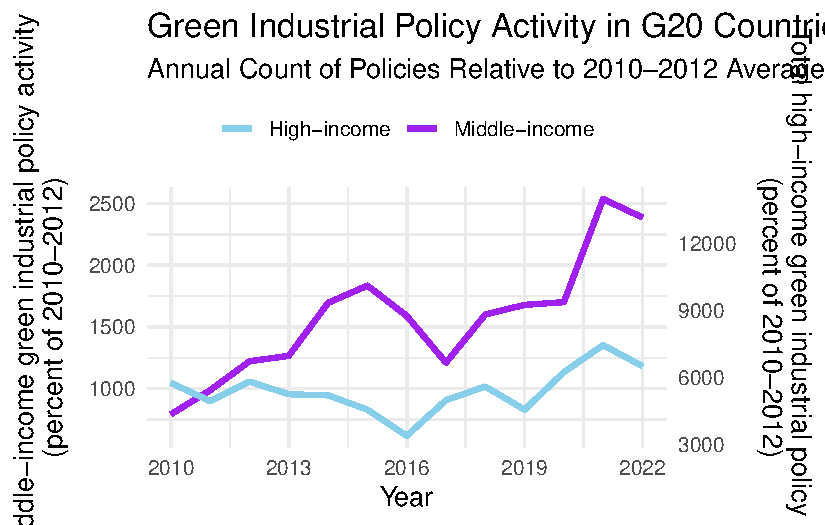
\includegraphics[keepaspectratio]{index_files/figure-pdf/unnamed-chunk-1-1.pdf}}

\begin{center}\rule{0.5\linewidth}{0.5pt}\end{center}

\section{Output of Figure 1
Replication}\label{output-of-figure-1-replication}

\begin{verbatim}
Loading required package: pacman
\end{verbatim}

\begin{verbatim}
The following packages have been unloaded:
pacman, janitor, haven, lubridate, forcats, stringr, dplyr, purrr, readr, tidyr, tibble, ggplot2, tidyverse
\end{verbatim}

\pandocbounded{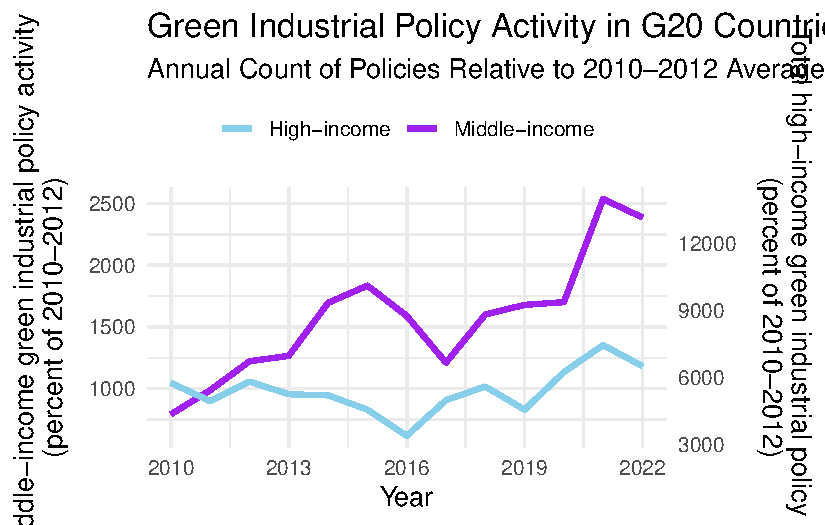
\includegraphics[keepaspectratio]{index_files/figure-pdf/unnamed-chunk-2-1.pdf}}

\begin{center}\rule{0.5\linewidth}{0.5pt}\end{center}

\section{Replication of Figure 2}\label{replication-of-figure-2}

\begin{itemize}
\tightlist
\item
  \textbf{Title:} Top Five Green Industrial Policy Instruments across
  G20 Economies by Income Group (2010--2022)
\item
  \textbf{What it shows:}

  \begin{itemize}
  \tightlist
  \item
    Distribution of green industrial policies by instrument type
    (e.g.~financial grant, state loan) -Comparison between High-income
    and Middle-income G20 countries -Focuses only on the top five most
    frequent instruments within each group -Measures are shown as shares
    of total green policy activity, normalized within each group
  \end{itemize}
\item
  \textbf{Axes:}

  \begin{itemize}
  \tightlist
  \item
    Left Y-axis: Income group (\emph{High-income} /
    \emph{Middle-income})\\
  \item
    Right Y-axis: Share of green policies by instrument type
  \end{itemize}
\end{itemize}

\begin{center}\rule{0.5\linewidth}{0.5pt}\end{center}

\section{Replication Figure}\label{replication-figure-1}

\begin{figure}[H]

{\centering 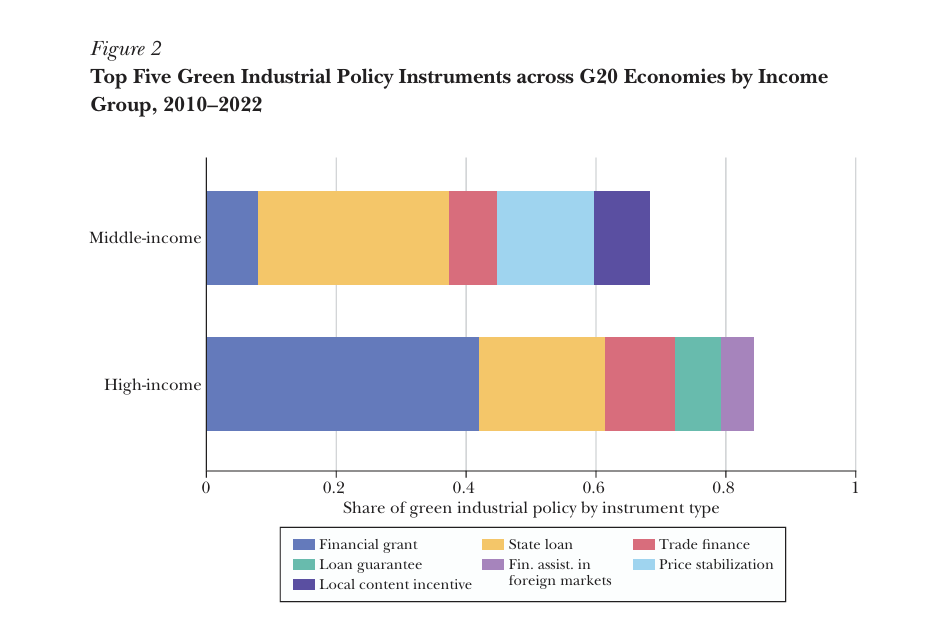
\includegraphics[width=1\linewidth,height=\textheight,keepaspectratio]{index_files/mediabag/figure_2.png}

}

\caption{Figure 2: Top five industrial policy intruments}

\end{figure}%

\begin{center}\rule{0.5\linewidth}{0.5pt}\end{center}

\section{\texorpdfstring{\textbf{Code Logic Summary -- Figure
2}}{Code Logic Summary -- Figure 2}}\label{code-logic-summary-figure-2}

\begin{itemize}
\item
  \textbf{Step 1: Load and prepare data}

  \begin{itemize}
  \tightlist
  \item
    Import \texttt{IP\_G20.dta} (policy dataset) and \texttt{wb.xlsx}
    (income classification)
  \item
    Standardize column names using \texttt{clean\_names()}
  \end{itemize}
\item
  \textbf{Step 2: Filter relevant policies}

  \begin{itemize}
  \tightlist
  \item
    Keep policies from 2010--2022 with non-missing descriptions
  \item
    These represent green or environmentally relevant measures
  \end{itemize}
\end{itemize}

\begin{center}\rule{0.5\linewidth}{0.5pt}\end{center}

\begin{itemize}
\item
  \textbf{Step 3: Assign income group}

  \begin{itemize}
  \tightlist
  \item
    Use a fixed list to classify countries as \emph{High-income} or
    \emph{Middle-income}
  \item
    Add this classification to each policy record
  \end{itemize}
\item
  \textbf{Step 4: Identify top 5 policy instruments}

  \begin{itemize}
  \tightlist
  \item
    Count frequency of each policy tool (\texttt{measure\_type})
  \item
    Select the top 5 most common types separately for each income group
  \end{itemize}
\item
  \textbf{Step 5: Compute usage shares}

  \begin{itemize}
  \tightlist
  \item
    Within each group, calculate how much each of the top 5 instruments
    was used
  \item
    Expressed as a share of total green policies in that group (0.0 to
    1.0)
  \end{itemize}
\end{itemize}

\begin{center}\rule{0.5\linewidth}{0.5pt}\end{center}

\begin{itemize}
\item
  \textbf{Step 6: Visualize with stacked bar chart}

  \begin{itemize}
  \tightlist
  \item
    Plot horizontal bars showing instrument composition by income group
  \item
    Use \texttt{coord\_flip()} to flip axes and
    \texttt{number\_format()} to show decimals
  \end{itemize}
\item
  \textbf{Step 7: Display output}

  \begin{itemize}
  \tightlist
  \item
    Render the plot with minimal styling and a grouped color legend
  \end{itemize}
\end{itemize}

\begin{center}\rule{0.5\linewidth}{0.5pt}\end{center}

\section{R Code for Replication}\label{r-code-for-replication-1}

\begin{Shaded}
\begin{Highlighting}[]
\CommentTok{\#  0) Load packages}
\ControlFlowTok{if}\NormalTok{ (}\SpecialCharTok{!}\FunctionTok{requireNamespace}\NormalTok{(}\StringTok{"pacman"}\NormalTok{, }\AttributeTok{quietly =} \ConstantTok{TRUE}\NormalTok{)) }\FunctionTok{install.packages}\NormalTok{(}\StringTok{"pacman"}\NormalTok{)}
\NormalTok{pacman}\SpecialCharTok{::}\FunctionTok{p\_load}\NormalTok{(}
\NormalTok{  haven,      }\CommentTok{\# for read\_dta()}
\NormalTok{  readxl,     }\CommentTok{\# for read\_xlsx()}
\NormalTok{  dplyr,      }
\NormalTok{  tidyr,}
\NormalTok{  ggplot2,}
\NormalTok{  scales,     }\CommentTok{\# for number\_format()}
\NormalTok{  janitor     }\CommentTok{\# for clean\_names()}
\NormalTok{)}
\CommentTok{\# {-}{-}{-}{-}{-}{-}{-}{-}{-}{-}{-}{-}{-}{-}{-}{-}{-}{-}{-}{-}{-}{-}{-}{-}{-}{-}{-}{-}{-}{-}{-}}
\CommentTok{\#  1) Ingest and clean{-}up }
\CommentTok{\# {-}{-}{-}{-}{-}{-}{-}{-}{-}{-}{-}{-}{-}{-}{-}{-}{-}{-}{-}{-}{-}{-}{-}{-}{-}{-}{-}{-}{-}{-}{-}}

\NormalTok{ip }\OtherTok{\textless{}{-}} \FunctionTok{read\_dta}\NormalTok{(}\StringTok{"E:/github/data science {-}presentation final/Data science presentation/Data{-}science{-}presentation{-}final/IP\_G20.dta"}\NormalTok{) }\SpecialCharTok{\%\textgreater{}\%}
  \FunctionTok{clean\_names}\NormalTok{()}

\CommentTok{\# Read and clean the income group Excel file}
\NormalTok{wb }\OtherTok{\textless{}{-}} \FunctionTok{read\_xlsx}\NormalTok{(}\StringTok{"E:/github/data science {-}presentation final/Data science presentation/Data{-}science{-}presentation{-}final/wb.xlsx"}\NormalTok{) }\SpecialCharTok{\%\textgreater{}\%}
  \FunctionTok{clean\_names}\NormalTok{()}

\CommentTok{\# {-}{-}{-}{-}{-}{-}{-}{-}{-}{-}{-}{-}{-}{-}{-}{-}{-}{-}{-}{-}{-}{-}{-}{-}{-}{-}{-}{-}{-}{-}{-}}
\CommentTok{\#  2) Filter green policies (2010–2022) and assign income group }
\CommentTok{\# {-}{-}{-}{-}{-}{-}{-}{-}{-}{-}{-}{-}{-}{-}{-}{-}{-}{-}{-}{-}{-}{-}{-}{-}{-}{-}{-}{-}{-}{-}{-}}
\NormalTok{high\_income\_countries }\OtherTok{\textless{}{-}} \FunctionTok{c}\NormalTok{(}
  \StringTok{"Australia"}\NormalTok{, }\StringTok{"Canada"}\NormalTok{, }\StringTok{"France"}\NormalTok{, }\StringTok{"Germany"}\NormalTok{, }\StringTok{"Italy"}\NormalTok{,}
  \StringTok{"Japan"}\NormalTok{, }\StringTok{"Republic of Korea"}\NormalTok{, }\StringTok{"United Kingdom"}\NormalTok{, }\StringTok{"United States"}\NormalTok{, }\StringTok{"European Union"}
\NormalTok{)}

\NormalTok{green }\OtherTok{\textless{}{-}}\NormalTok{ ip }\SpecialCharTok{\%\textgreater{}\%}
  \FunctionTok{filter}\NormalTok{(}
    \SpecialCharTok{!}\FunctionTok{is.na}\NormalTok{(measure\_description\_tokens),}
\NormalTok{    announced\_year }\SpecialCharTok{\textgreater{}=} \DecValTok{2010}\NormalTok{,}
\NormalTok{    announced\_year }\SpecialCharTok{\textless{}=} \DecValTok{2022}
\NormalTok{  ) }\SpecialCharTok{\%\textgreater{}\%}
  \FunctionTok{mutate}\NormalTok{(}
    \AttributeTok{income\_group =} \FunctionTok{if\_else}\NormalTok{(}
\NormalTok{      country\_std }\SpecialCharTok{\%in\%}\NormalTok{ high\_income\_countries,}
      \StringTok{"High{-}income"}\NormalTok{,}
      \StringTok{"Middle{-}income"}
\NormalTok{    )}
\NormalTok{  )}
\CommentTok{\# {-}{-}{-}{-}{-}{-}{-}{-}{-}{-}{-}{-}{-}{-}{-}{-}{-}{-}{-}{-}{-}{-}{-}{-}{-}{-}{-}{-}{-}{-}{-}}
\CommentTok{\# 3) Identify top 5 instrument types per income group }
\CommentTok{\# {-}{-}{-}{-}{-}{-}{-}{-}{-}{-}{-}{-}{-}{-}{-}{-}{-}{-}{-}{-}{-}{-}{-}{-}{-}{-}{-}{-}{-}{-}{-}}
\NormalTok{top5 }\OtherTok{\textless{}{-}}\NormalTok{ green }\SpecialCharTok{\%\textgreater{}\%}
  \FunctionTok{count}\NormalTok{(income\_group, measure\_type, }\AttributeTok{name =} \StringTok{"n"}\NormalTok{) }\SpecialCharTok{\%\textgreater{}\%}
  \FunctionTok{group\_by}\NormalTok{(income\_group) }\SpecialCharTok{\%\textgreater{}\%}
  \FunctionTok{slice\_max}\NormalTok{(n, }\AttributeTok{n =} \DecValTok{5}\NormalTok{) }\SpecialCharTok{\%\textgreater{}\%}
  \FunctionTok{pull}\NormalTok{(measure\_type) }\SpecialCharTok{\%\textgreater{}\%}
  \FunctionTok{unique}\NormalTok{()}
\CommentTok{\# {-}{-}{-}{-}{-}{-}{-}{-}{-}{-}{-}{-}{-}{-}{-}{-}{-}{-}{-}{-}{-}{-}{-}{-}{-}{-}{-}{-}{-}{-}{-}}
\CommentTok{\#  4) Compute shares of top 5 instruments }
\CommentTok{\# {-}{-}{-}{-}{-}{-}{-}{-}{-}{-}{-}{-}{-}{-}{-}{-}{-}{-}{-}{-}{-}{-}{-}{-}{-}{-}{-}{-}{-}{-}{-}}
\NormalTok{plot\_df }\OtherTok{\textless{}{-}}\NormalTok{ green }\SpecialCharTok{\%\textgreater{}\%}
  \FunctionTok{filter}\NormalTok{(measure\_type }\SpecialCharTok{\%in\%}\NormalTok{ top5) }\SpecialCharTok{\%\textgreater{}\%}
  \FunctionTok{count}\NormalTok{(income\_group, measure\_type, }\AttributeTok{name =} \StringTok{"n"}\NormalTok{) }\SpecialCharTok{\%\textgreater{}\%}
  \FunctionTok{group\_by}\NormalTok{(income\_group) }\SpecialCharTok{\%\textgreater{}\%}
  \FunctionTok{mutate}\NormalTok{(}\AttributeTok{share =}\NormalTok{ n }\SpecialCharTok{/} \FunctionTok{sum}\NormalTok{(n)) }\SpecialCharTok{\%\textgreater{}\%}
  \FunctionTok{ungroup}\NormalTok{()}
\CommentTok{\# {-}{-}{-}{-}{-}{-}{-}{-}{-}{-}{-}{-}{-}{-}{-}{-}{-}{-}{-}{-}{-}{-}{-}{-}{-}{-}{-}{-}{-}{-}{-}}
\CommentTok{\#  5) Build the horizontal stacked bar plot}
\CommentTok{\# {-}{-}{-}{-}{-}{-}{-}{-}{-}{-}{-}{-}{-}{-}{-}{-}{-}{-}{-}{-}{-}{-}{-}{-}{-}{-}{-}{-}{-}{-}{-}}
\NormalTok{p }\OtherTok{\textless{}{-}} \FunctionTok{ggplot}\NormalTok{(plot\_df, }\FunctionTok{aes}\NormalTok{(}
    \AttributeTok{x =}\NormalTok{ income\_group,}
    \AttributeTok{y =}\NormalTok{ share,}
    \AttributeTok{fill =}\NormalTok{ measure\_type}
\NormalTok{  )) }\SpecialCharTok{+}
  \FunctionTok{geom\_col}\NormalTok{(}\AttributeTok{position =} \StringTok{"fill"}\NormalTok{, }\AttributeTok{width =} \FloatTok{0.6}\NormalTok{) }\SpecialCharTok{+}
  \FunctionTok{coord\_flip}\NormalTok{() }\SpecialCharTok{+}
  \FunctionTok{scale\_y\_continuous}\NormalTok{(}
    \AttributeTok{breaks =} \FunctionTok{seq}\NormalTok{(}\DecValTok{0}\NormalTok{, }\DecValTok{1}\NormalTok{, }\AttributeTok{by =} \FloatTok{0.2}\NormalTok{),}
    \AttributeTok{labels =} \FunctionTok{number\_format}\NormalTok{(}\AttributeTok{accuracy =} \FloatTok{0.1}\NormalTok{),}
    \AttributeTok{expand =} \FunctionTok{expansion}\NormalTok{(}\AttributeTok{mult =} \FunctionTok{c}\NormalTok{(}\DecValTok{0}\NormalTok{, }\DecValTok{0}\NormalTok{))}
\NormalTok{  ) }\SpecialCharTok{+}
  \FunctionTok{labs}\NormalTok{(}
    \AttributeTok{title =} \StringTok{"Top Five Green Industrial Policy Instruments Across G20 Economies}\SpecialCharTok{\textbackslash{}n}\StringTok{by Income Group, 2010–2022"}\NormalTok{,}
    \AttributeTok{x =} \ConstantTok{NULL}\NormalTok{,}
    \AttributeTok{y =} \StringTok{"Share of green industrial policy by instrument type"}\NormalTok{,}
    \AttributeTok{fill =} \StringTok{"Instrument Type"}
\NormalTok{  ) }\SpecialCharTok{+}
  \FunctionTok{theme\_minimal}\NormalTok{(}\AttributeTok{base\_size =} \DecValTok{14}\NormalTok{) }\SpecialCharTok{+}
  \FunctionTok{theme}\NormalTok{(}
    \AttributeTok{plot.title      =} \FunctionTok{element\_text}\NormalTok{(}\AttributeTok{face =} \StringTok{"bold"}\NormalTok{, }\AttributeTok{size =} \DecValTok{16}\NormalTok{, }\AttributeTok{hjust =} \DecValTok{0}\NormalTok{),}
    \AttributeTok{axis.text.y     =} \FunctionTok{element\_text}\NormalTok{(}\AttributeTok{size =} \DecValTok{12}\NormalTok{),}
    \AttributeTok{panel.grid.minor =} \FunctionTok{element\_blank}\NormalTok{(),}
    \AttributeTok{legend.position =} \StringTok{"bottom"}\NormalTok{,}
    \AttributeTok{legend.key.size =} \FunctionTok{unit}\NormalTok{(}\FloatTok{0.7}\NormalTok{, }\StringTok{"lines"}\NormalTok{)}
\NormalTok{  )}
\CommentTok{\# {-}{-}{-}{-}{-}{-}{-}{-}{-}{-}{-}{-}{-}{-}{-}{-}{-}{-}{-}{-}{-}{-}{-}{-}{-}{-}{-}{-}{-}{-}{-}}
\CommentTok{\# ️ 6) Display the plot}
\CommentTok{\# {-}{-}{-}{-}{-}{-}{-}{-}{-}{-}{-}{-}{-}{-}{-}{-}{-}{-}{-}{-}{-}{-}{-}{-}{-}{-}{-}{-}{-}{-}{-}}
\FunctionTok{print}\NormalTok{(p)}
\end{Highlighting}
\end{Shaded}

\pandocbounded{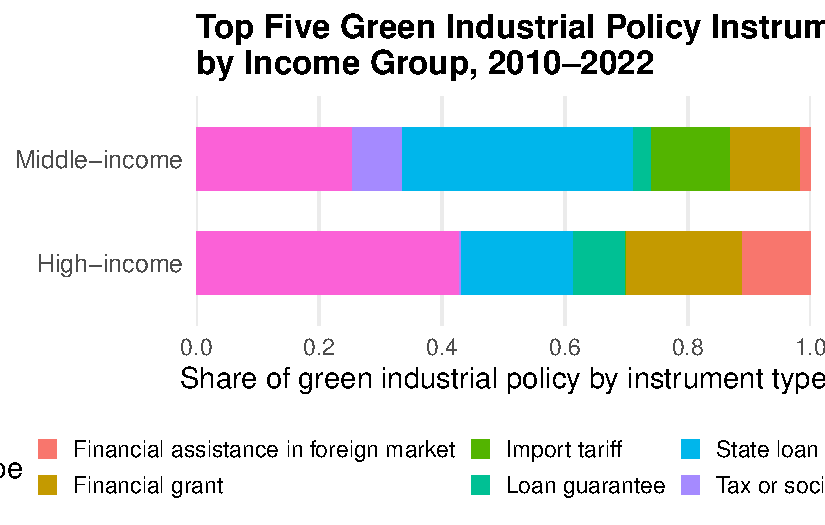
\includegraphics[keepaspectratio]{index_files/figure-pdf/unnamed-chunk-3-1.pdf}}

\section{Output of Figure 2
Replication}\label{output-of-figure-2-replication}

\begin{Shaded}
\begin{Highlighting}[]
\ControlFlowTok{if}\NormalTok{ (}\SpecialCharTok{!}\FunctionTok{requireNamespace}\NormalTok{(}\StringTok{"pacman"}\NormalTok{, }\AttributeTok{quietly =} \ConstantTok{TRUE}\NormalTok{)) }\FunctionTok{install.packages}\NormalTok{(}\StringTok{"pacman"}\NormalTok{)}
\NormalTok{pacman}\SpecialCharTok{::}\FunctionTok{p\_load}\NormalTok{(}
\NormalTok{  haven,      }\CommentTok{\# for read\_dta()}
\NormalTok{  readxl,     }\CommentTok{\# for read\_xlsx()}
\NormalTok{  dplyr,      }
\NormalTok{  tidyr,}
\NormalTok{  ggplot2,}
\NormalTok{  scales,     }\CommentTok{\# for number\_format()}
\NormalTok{  janitor     }\CommentTok{\# for clean\_names()}
\NormalTok{)}
\CommentTok{\# {-}{-}{-}{-}{-}{-}{-}{-}{-}{-}{-}{-}{-}{-}{-}{-}{-}{-}{-}{-}{-}{-}{-}{-}{-}{-}{-}{-}{-}{-}{-}}
\CommentTok{\#  1) Ingest and clean{-}up}
\CommentTok{\# {-}{-}{-}{-}{-}{-}{-}{-}{-}{-}{-}{-}{-}{-}{-}{-}{-}{-}{-}{-}{-}{-}{-}{-}{-}{-}{-}{-}{-}{-}{-}}

\NormalTok{ip }\OtherTok{\textless{}{-}} \FunctionTok{read\_dta}\NormalTok{(}\StringTok{"E:/github/data science {-}presentation final/Data science presentation/Data{-}science{-}presentation{-}final/IP\_G20.dta"}\NormalTok{) }\SpecialCharTok{\%\textgreater{}\%}
  \FunctionTok{clean\_names}\NormalTok{()}

\CommentTok{\# Read and clean the income group Excel file}
\NormalTok{wb }\OtherTok{\textless{}{-}} \FunctionTok{read\_xlsx}\NormalTok{(}\StringTok{"E:/github/data science {-}presentation final/Data science presentation/Data{-}science{-}presentation{-}final/wb.xlsx"}\NormalTok{) }\SpecialCharTok{\%\textgreater{}\%}
  \FunctionTok{clean\_names}\NormalTok{()}

\CommentTok{\# {-}{-}{-}{-}{-}{-}{-}{-}{-}{-}{-}{-}{-}{-}{-}{-}{-}{-}{-}{-}{-}{-}{-}{-}{-}{-}{-}{-}{-}{-}{-}}
\CommentTok{\#  2) Filter green policies (2010–2022) and assign income group }
\CommentTok{\# {-}{-}{-}{-}{-}{-}{-}{-}{-}{-}{-}{-}{-}{-}{-}{-}{-}{-}{-}{-}{-}{-}{-}{-}{-}{-}{-}{-}{-}{-}{-}}
\NormalTok{high\_income\_countries }\OtherTok{\textless{}{-}} \FunctionTok{c}\NormalTok{(}
  \StringTok{"Australia"}\NormalTok{, }\StringTok{"Canada"}\NormalTok{, }\StringTok{"France"}\NormalTok{, }\StringTok{"Germany"}\NormalTok{, }\StringTok{"Italy"}\NormalTok{,}
  \StringTok{"Japan"}\NormalTok{, }\StringTok{"Republic of Korea"}\NormalTok{, }\StringTok{"United Kingdom"}\NormalTok{, }\StringTok{"United States"}\NormalTok{, }\StringTok{"European Union"}
\NormalTok{)}

\NormalTok{green }\OtherTok{\textless{}{-}}\NormalTok{ ip }\SpecialCharTok{\%\textgreater{}\%}
  \FunctionTok{filter}\NormalTok{(}
    \SpecialCharTok{!}\FunctionTok{is.na}\NormalTok{(measure\_description\_tokens),}
\NormalTok{    announced\_year }\SpecialCharTok{\textgreater{}=} \DecValTok{2010}\NormalTok{,}
\NormalTok{    announced\_year }\SpecialCharTok{\textless{}=} \DecValTok{2022}
\NormalTok{  ) }\SpecialCharTok{\%\textgreater{}\%}
  \FunctionTok{mutate}\NormalTok{(}
    \AttributeTok{income\_group =} \FunctionTok{if\_else}\NormalTok{(}
\NormalTok{      country\_std }\SpecialCharTok{\%in\%}\NormalTok{ high\_income\_countries,}
      \StringTok{"High{-}income"}\NormalTok{,}
      \StringTok{"Middle{-}income"}
\NormalTok{    )}
\NormalTok{  )}

\CommentTok{\# {-}{-}{-}{-}{-}{-}{-}{-}{-}{-}{-}{-}{-}{-}{-}{-}{-}{-}{-}{-}{-}{-}{-}{-}{-}{-}{-}{-}{-}{-}{-}}
\CommentTok{\# 3) Identify top 5 instrument types per income group}
\CommentTok{\# {-}{-}{-}{-}{-}{-}{-}{-}{-}{-}{-}{-}{-}{-}{-}{-}{-}{-}{-}{-}{-}{-}{-}{-}{-}{-}{-}{-}{-}{-}{-}}
\NormalTok{top5 }\OtherTok{\textless{}{-}}\NormalTok{ green }\SpecialCharTok{\%\textgreater{}\%}
  \FunctionTok{count}\NormalTok{(income\_group, measure\_type, }\AttributeTok{name =} \StringTok{"n"}\NormalTok{) }\SpecialCharTok{\%\textgreater{}\%}
  \FunctionTok{group\_by}\NormalTok{(income\_group) }\SpecialCharTok{\%\textgreater{}\%}
  \FunctionTok{slice\_max}\NormalTok{(n, }\AttributeTok{n =} \DecValTok{5}\NormalTok{) }\SpecialCharTok{\%\textgreater{}\%}
  \FunctionTok{pull}\NormalTok{(measure\_type) }\SpecialCharTok{\%\textgreater{}\%}
  \FunctionTok{unique}\NormalTok{()}

\CommentTok{\# {-}{-}{-}{-}{-}{-}{-}{-}{-}{-}{-}{-}{-}{-}{-}{-}{-}{-}{-}{-}{-}{-}{-}{-}{-}{-}{-}{-}{-}{-}{-}}
\CommentTok{\#  4) Compute shares of top 5 instruments}
\CommentTok{\# {-}{-}{-}{-}{-}{-}{-}{-}{-}{-}{-}{-}{-}{-}{-}{-}{-}{-}{-}{-}{-}{-}{-}{-}{-}{-}{-}{-}{-}{-}{-}}
\NormalTok{plot\_df }\OtherTok{\textless{}{-}}\NormalTok{ green }\SpecialCharTok{\%\textgreater{}\%}
  \FunctionTok{filter}\NormalTok{(measure\_type }\SpecialCharTok{\%in\%}\NormalTok{ top5) }\SpecialCharTok{\%\textgreater{}\%}
  \FunctionTok{count}\NormalTok{(income\_group, measure\_type, }\AttributeTok{name =} \StringTok{"n"}\NormalTok{) }\SpecialCharTok{\%\textgreater{}\%}
  \FunctionTok{group\_by}\NormalTok{(income\_group) }\SpecialCharTok{\%\textgreater{}\%}
  \FunctionTok{mutate}\NormalTok{(}\AttributeTok{share =}\NormalTok{ n }\SpecialCharTok{/} \FunctionTok{sum}\NormalTok{(n)) }\SpecialCharTok{\%\textgreater{}\%}
  \FunctionTok{ungroup}\NormalTok{()}

\CommentTok{\# {-}{-}{-}{-}{-}{-}{-}{-}{-}{-}{-}{-}{-}{-}{-}{-}{-}{-}{-}{-}{-}{-}{-}{-}{-}{-}{-}{-}{-}{-}{-}}
\CommentTok{\#  5) Build the horizontal stacked bar plot}
\CommentTok{\# {-}{-}{-}{-}{-}{-}{-}{-}{-}{-}{-}{-}{-}{-}{-}{-}{-}{-}{-}{-}{-}{-}{-}{-}{-}{-}{-}{-}{-}{-}{-}}
\NormalTok{p }\OtherTok{\textless{}{-}} \FunctionTok{ggplot}\NormalTok{(plot\_df, }\FunctionTok{aes}\NormalTok{(}
    \AttributeTok{x =}\NormalTok{ income\_group,}
    \AttributeTok{y =}\NormalTok{ share,}
    \AttributeTok{fill =}\NormalTok{ measure\_type}
\NormalTok{  )) }\SpecialCharTok{+}
  \FunctionTok{geom\_col}\NormalTok{(}\AttributeTok{position =} \StringTok{"fill"}\NormalTok{, }\AttributeTok{width =} \FloatTok{0.6}\NormalTok{) }\SpecialCharTok{+}
  \FunctionTok{coord\_flip}\NormalTok{() }\SpecialCharTok{+}
  \FunctionTok{scale\_y\_continuous}\NormalTok{(}
    \AttributeTok{breaks =} \FunctionTok{seq}\NormalTok{(}\DecValTok{0}\NormalTok{, }\DecValTok{1}\NormalTok{, }\AttributeTok{by =} \FloatTok{0.2}\NormalTok{),}
    \AttributeTok{labels =} \FunctionTok{number\_format}\NormalTok{(}\AttributeTok{accuracy =} \FloatTok{0.1}\NormalTok{),}
    \AttributeTok{expand =} \FunctionTok{expansion}\NormalTok{(}\AttributeTok{mult =} \FunctionTok{c}\NormalTok{(}\DecValTok{0}\NormalTok{, }\DecValTok{0}\NormalTok{))}
\NormalTok{  ) }\SpecialCharTok{+}
  \FunctionTok{labs}\NormalTok{(}
    \AttributeTok{title =} \StringTok{"Top Five Green Industrial Policy Instruments Across G20 Economies}\SpecialCharTok{\textbackslash{}n}\StringTok{by Income Group, 2010–2022"}\NormalTok{,}
    \AttributeTok{x =} \ConstantTok{NULL}\NormalTok{,}
    \AttributeTok{y =} \StringTok{"Share of green industrial policy by instrument type"}\NormalTok{,}
    \AttributeTok{fill =} \StringTok{"Instrument Type"}
\NormalTok{  ) }\SpecialCharTok{+}
  \FunctionTok{theme\_minimal}\NormalTok{(}\AttributeTok{base\_size =} \DecValTok{14}\NormalTok{) }\SpecialCharTok{+}
  \FunctionTok{theme}\NormalTok{(}
    \AttributeTok{plot.title      =} \FunctionTok{element\_text}\NormalTok{(}\AttributeTok{face =} \StringTok{"bold"}\NormalTok{, }\AttributeTok{size =} \DecValTok{16}\NormalTok{, }\AttributeTok{hjust =} \DecValTok{0}\NormalTok{),}
    \AttributeTok{axis.text.y     =} \FunctionTok{element\_text}\NormalTok{(}\AttributeTok{size =} \DecValTok{12}\NormalTok{),}
    \AttributeTok{panel.grid.minor =} \FunctionTok{element\_blank}\NormalTok{(),}
    \AttributeTok{legend.position =} \StringTok{"bottom"}\NormalTok{,}
    \AttributeTok{legend.key.size =} \FunctionTok{unit}\NormalTok{(}\FloatTok{0.7}\NormalTok{, }\StringTok{"lines"}\NormalTok{)}
\NormalTok{  )}
\CommentTok{\# {-}{-}{-}{-}{-}{-}{-}{-}{-}{-}{-}{-}{-}{-}{-}{-}{-}{-}{-}{-}{-}{-}{-}{-}{-}{-}{-}{-}{-}{-}{-}}
\CommentTok{\# ️ 6) Display the plot}
\CommentTok{\# {-}{-}{-}{-}{-}{-}{-}{-}{-}{-}{-}{-}{-}{-}{-}{-}{-}{-}{-}{-}{-}{-}{-}{-}{-}{-}{-}{-}{-}{-}{-}}
\FunctionTok{print}\NormalTok{(p)}
\end{Highlighting}
\end{Shaded}

\pandocbounded{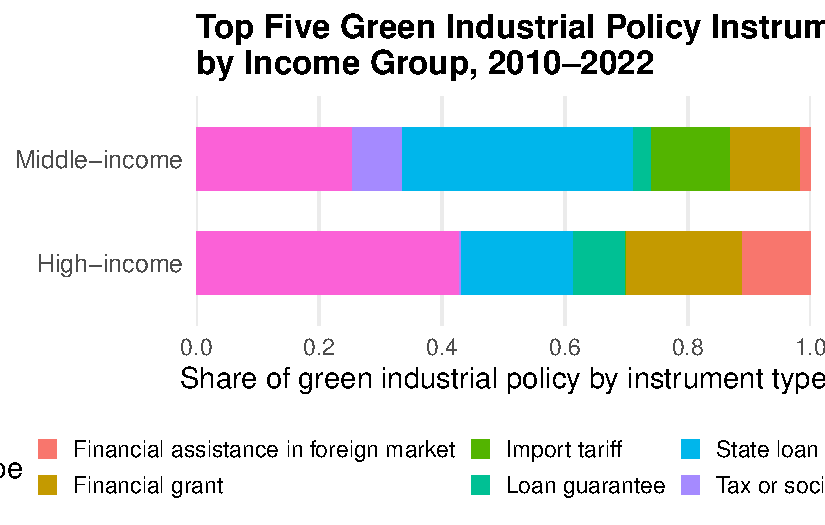
\includegraphics[keepaspectratio]{index_files/figure-pdf/unnamed-chunk-4-1.pdf}}

\section{Challenges faces}\label{challenges-faces}

\begin{itemize}
\item
  Uploaded local data files to GitHub and linked using raw URLs so
  others could run the code.
\item
  Replaced \texttt{percent\_format()} with \texttt{number\_format()} to
  show axis labels as decimals.
\item
  Renamed output to \texttt{index.html} so GitHub Pages would display
  the updated version.
\end{itemize}

\begin{center}\rule{0.5\linewidth}{0.5pt}\end{center}

\section{Future Work with this
Replication}\label{future-work-with-this-replication}

\begin{itemize}
\tightlist
\item
  \textbf{Clean and verify all country names}

  \begin{itemize}
  \tightlist
  \item
    Match them correctly with World Bank data to fix missing values
  \end{itemize}
\item
  \textbf{Improve keyword filtering}

  \begin{itemize}
  \tightlist
  \item
    Refine how we identify green policies using better or more complete
    keywords
  \end{itemize}
\item
  \textbf{Match Stata version exactly}

  \begin{itemize}
  \tightlist
  \item
    Compare our R code outputs with the original Stata graphs for full
    accuracy
  \end{itemize}
\end{itemize}

\begin{center}\rule{0.5\linewidth}{0.5pt}\end{center}

\begin{itemize}
\tightlist
\item
  \textbf{Check missing data}

  \begin{itemize}
  \tightlist
  \item
    Investigate why some years or countries have fewer policies than
    expected
  \end{itemize}
\item
  \textbf{Automate income group assignment}

  \begin{itemize}
  \tightlist
  \item
    Instead of manual grouping, use official classification files from
    the World Bank
  \end{itemize}
\end{itemize}




\end{document}
